\chapter{\label{chap:tsp}The Hamiltonian Path and Travelling Salesman Problems}

% \begin{abstract}
% The Hamiltonian Cycle Problem (HCP) and Travelling Salesman Problem (TSP) are long-standing and well-known NP-hard problems.  The \gls{hpp} is concerned with finding paths through a given graph such that those paths visit each node exactly once after the start, and end where they began (i.e., Hamiltonian cycles).  The TSP builds on the \gls{hpp} and is concerned with computing the lowest cost Hamiltonian cycle on a weighted (di)graph.  Many solutions to these problems exist, including some from the perspective of P~systems.  For the TSP however, almost all these papers have combined membrane computing with other approaches for approximate solution algorithms, which is surprising given the plethora of P~systems solutions to the \gls{hpp}.  A recent paper presented a brute-force style P~systems solution to the TSP with a time complexity of \(\mathcal{O}(n^2)\), exploiting the ability of P~systems to reduce time complexity in exchange for space complexity, but the resultant system had a fairly high number of rules, around 50.  Inspired by this paper, and seeking a more concise representation of an exact brute-force TSP algorithm, we have devised a P~systems algorithm based on cP~systems (P~systems with Complex Objects) which requires five rules and takes \(n + 3\) steps.  We first provide some background on cP~systems and demonstrate a fast new cP~systems method to find the minimum of a multiset, then describe our solution to the \gls{hpp}, and build on that for our TSP algorithm.  This paper describes said algorithms, and provides an example application of our TSP algorithm to a given graph and a digraph variant.
% \end{abstract}

% \begin{keywords}
% cP~systems, P~systems, Prolog terms and unification, Travelling Salesman Problem, Hamiltonian Cycle Problem
% \end{keywords}


%-------------------------------------------------

\section{Background}

The \gls{hpp} is a long-standing, well-known computationally hard (NP-hard) problem in Computer Science and related fields.  The problem consists of trying to determine whether for a given graph (digraph) there exists a traversal of the graph in which each node (vertex) is visited exactly once.  Depending on the particular problem at hand, the starting and/or ending node may or may not be arbitrarily selected.  Intrinsically linked, and arguably more useful, is \emph{describing} such a Hamiltonian path -- describing such a path proves the existence of it, and allows for its potential use in practical applications.  The \gls{hcp} is a closely related variant, in which the Hamiltonian path must also be a cycle, i.e., the final node (vertex) in the path is the same as the starting one, such that every node (vertex) is visited exactly once after the start.

The \gls{hpp}/\gls{hcp} has been examined before through the lens of \gls{ps}, with different variants of \gls{ps} used such as \gls{tlps} \cite{Martin-Vide2003}, P~systems with active membranes \cite{Pan2006,Song2013}, Recogniser P~systems \cite{Chen2009}, Asynchronous P~systems \cite{Tagawa2012} and \gls{snps} \cite{Xue2013}.  Jim\'enez \textit{et al.} used the \gls{hpp} as an example computation when discussing complexity classes in \gls{ps} \cite{Jimenez2003}.  In fact, it was demonstrated relatively early in the history of \gls{ps} that some variants at least could be used to solve the \gls{hpp} in linear time \cite{Mutyam2001}.  This last approach, using \gls{ps} with membrane creation, is arguably the closest to our approach, which involves the instantiation of subcells (complex objects).

The \gls{tsp} is an extension upon the \gls{hcp}, and is about finding the minimum cost Hamiltonian cycle in a \emph{weighted} graph.  It has been described as analogous to finding the shortest route for a travelling salesman to visit multiple cities in one trip (whence the name).  The problem is arguably the most useful of the three to solve in practice, and has been studied extensively, spawning many papers, dissertations and books on the topic (e.g. \cite{Smith2017,Ezugwu2017,Cook2012,Applegate2006} amongst many, many others).  A variety of sophisticated algorithms have been developed to solve the problem efficiently, in either the exact or approximate case.  This chapter does not seek overturn this prior body of work.  Instead, it seeks to address the problem from a cP~systems perspective.  Note that we discuss here the \emph{optimisation} form of the \gls{tsp}, which is NP-Hard but not NP-Complete, and not the \emph{decision} form of the \gls{tsp}, which is NP-Complete.\footnote{See for example \url{https://www.ibm.com/developerworks/community/blogs/jfp/entry/no_the_tsp_isn_t_np_complete?lang=en} for an interesting but informal discussion of the difference.}%  This demonstrates that cP~systems, and presumably other forms of \gls{ps} too, are capable of solving in polynomial time problems for which there is no known traditional polynomial-time verification% -- a requirement for NP-Complete.

A small amount of work has been done on the \gls{tsp} from the perspective of membrane computing, beginning with the work of Nishida \cite{Nishida2006}, who used a combination of a membrane structure and pre-existing methods to search for an approximate solution in a space of solutions to the \gls{tsp} for a given digraph.  Others built on this approach by integrating techniques such as Genetic Algorithms \cite{Manalastas2013,He2014}, Ant Colony Optimisation \cite{Zhang2011} and Active Evolution \cite{Song2015}, along with more complex approaches for multiple salesman problems \cite{He2015}.  A paper by Chen \textit{et al.} \cite{Chen2011} was apparently also written on the topic, but no copy of that paper could be located.

Surprisingly however, given the multitude of solutions already demonstrated for the \gls{hcp}, all these \gls{tsp} papers have been written from the perspective of approximate solutions to the \gls{tsp}.  They typically take an approach of using membranes to divide up the search space of potential solutions, whilst applying other pre-existing techniques to the process.  These papers have used membranes to structure a search space, but in our view have not fully embraced the \gls{ps} model, e.g. none of them have specified typical \gls{ps} rewriting rules, instead applying other techniques within the subcells, and using \gls{ps} rules only to move potential solutions between cells.  More recently however, Guo and Dai presented a paper on solving the \gls{tsp} in the exact case using \gls{clps} \cite{Guo2017}, requiring roughly 50 rules.  By exploiting the well-known property of many \gls{ps} variants that time complexity can often be exchanged for space and/or processing complexity \cite{Paun1999,Paun2002a,Jimenez2003,Song2017}, the authors derived a \gls{ps} algorithm that can solve the \gls{tsp} in \(\mathcal{O}(n^2)\) time.

% Inspired by \cite{Guo2017}, we derive a cP~systems algorithm for solving the \gls{tsp}, fully exploiting the power of \gls{ps}' theoretical infinite resources, as well as the compactness of representation of cP~systems.  Such systems have been described extensively in prior papers, in particular most recently in \cite{Nicolescu2018a}.  The use of cP~systems' generic maximally parallel multiset rewriting rules, and Prolog-like terms and unification, increases the expressive power of each rule, enabling us to specify here a fixed-size ruleset of five rules, applicable to digraphs of any size or complexity.   Further, our algorithm can solve any instance in \(n + 3\) steps, where \(n\) is the number of vertices in the digraph (thus the time complexity of our algorithm is \(\mathcal{O}(n)\)).  This paper mainly focuses on the \gls{tsp}, though we begin with a solution to the less-complicated \gls{hpp}, then expand that to the \gls{hcp}, and then expand upon that to solve the \gls{tsp}.  In the latter two cases, only relatively minor modifications to our rules are required at each step in order to take account of the stricter requirements of the problem.

Inspired by \cite{Guo2017}, we derive a cP~systems algorithm for solving the \gls{tsp}, fully exploiting the power of \gls{ps}' theoretical infinite resources, as well as the compactness of representation of cP~systems.  The use of cP~systems' generic maximally parallel multiset rewriting rules, and Prolog-like terms and unification, increases the expressive power of each rule, enabling us to specify here a fixed-size ruleset of five rules, applicable to digraphs of any size or complexity.   Further, our algorithm can solve any instance in \(n + 3\) steps, where \(n\) is the number of vertices in the digraph (thus the time complexity of our algorithm is \(\mathcal{O}(n)\)).  This chapter mainly focuses on the \gls{tsp}, though we begin with a solution to the less-complicated \gls{hpp}, then expand that to the \gls{hcp}, and then expand upon that to solve the \gls{tsp}.  In the latter two cases, only relatively minor modifications to our rules are required at each step in order to take account of the stricter requirements of the problem.

% For the sake of space, we hereafter assume that the reader is familiar with the basic concepts of \gls{ps} (see \cite{Paun2009} for a good, if slightly old, introduction to \gls{ps}), and the \gls{hcp} \& the \gls{tsp}.  In \autoref{sec:tsp:cpsystems} we present revised and improved material from previous papers that describes key aspects of cP~systems relevant to this paper (the reader is referred to \cite{Nicolescu2014a,RN-HW-ROMJIST14,Nicolescu2018a} also), before setting out a new cP~systems method for finding the minimum of a multiset in a single step, which requires two rules.  Our algorithms, and in particular the rules for them, are presented for the \gls{hpp} \& \gls{hcp} and \gls{tsp} cases respectively in \autoref{sec:tsp:algohpp} and \autoref{sec:tsp:algotsp}.  We provide worked examples for the \gls{tsp} in \autoref{sec:tsp:example}, applying our algorithm to a specific weighted graph and a modified digraph version of it.  We then consider some potential variations on the algorithm for differing results in \autoref{sec:tsp:variations}.  Finally, we briefly discuss simulations of the \gls{tsp} system written in SWI-Prolog, F\# and Erlang in \autoref{sec:tsp:simulation}.

Our algorithms, and in particular the rules for them, are presented for the \gls{hpp} \& \gls{hcp} and \gls{tsp} cases respectively in \autoref{sec:tsp:algohpp} and \autoref{sec:tsp:algotsp}.  We provide worked examples for the \gls{tsp} in \autoref{sec:tsp:example}, applying our algorithm to a specific weighted graph and a modified digraph version of it.  We then consider some potential variations on the algorithm for differing results in \autoref{sec:tsp:variations}.  Finally, we briefly discuss simulations of the \gls{tsp} system written in SWI-Prolog, F\# and Erlang in \autoref{sec:tsp:simulation}.
% \subsection{\label{sec:tsp:cpsystems}\texorpdfstring{\gls{cps}}{cP systems} : \texorpdfstring{\gls{ps}}{P systems} with Complex Symbols}
% --------------------------------------------------

In the interests of self-containment, we present here some material describing the background of \gls{cps}, for the benefit of readers as yet unfamiliar with the topic.  More extensive presentation of \gls{cps} has appeared most recently in \cite{Nicolescu2018}, and it is recommended that the interested reader peruse that paper as well.  There are two notable additions shown here that are not in \cite{Nicolescu2018}, however: the stronger semantics for inhibitors, to fully implement logical negation; and the minimum-finding algorithm explained in \autoref{sec-min}, used in solving the \gls{tsp}.  We wish to point out that, while \gls{cps} is transitively bio-inspired through its basis in \gls{ps}, it has not been developed with the aim of simulating or modelling real-world biology, and instead is intended as a useful theoretical model for computation.

\subsubsection{Complex symbols as subcells}

\emph{Complex symbols} or \emph{subcells}, 
play the roles of cellular micro-compartments or substructures,
such as organelles, vesicles or cytoophidium assemblies (``snakes''),
which are embedded in cells or travel between cells, 
but without having the full processing power of a complete cell.
In our proposal, \emph{subcells} represent nested labelled data compartments
with no processing power of their own;
instead, they are acted upon by the rules of their enclosing cells.

Our basic vocabulary consists of \emph{atoms} and \emph{variables}, 
collectively known as \emph{simple symbols}.
\emph{Complex symbols} are similar to Prolog-like \emph{first-order terms}, 
recursively built from \emph{multisets} of atoms and variables.
Together, complex symbols and simple symbols (atoms, variables) are called \emph{symbols},
%We omit a formal grammar for them here.
and can be defined by the following formal grammar:

\begin{framed}
\vspace{-0.5cm}
\begin{small}
\begin{alltt}
    <symbol> ::= <atom> | <variable> | <term> 
    <term> ::= <functor> '(' <argument> ')'
    <functor> ::= <atom>
    <argument> ::= \(\lambda\) | ( <symbol> )+
\end{alltt}
\end{small}
\vspace{-0.5cm}
\end{framed}

\emph{Atoms} are typically denoted by lower case letters (or, occasionally, digits), 
such as $a$, $b$, $c$, \(\cpundig\). 
\emph{Variables} are typically denoted by uppercase letters, 
such as $X$, $Y$, $Z$.
\emph{Functors} are term (subcell) labels; here functors can only be atoms, not variables.

For improved readability, we also consider \emph{anonymous variables}, which are denoted by underscores (``$\_$'').
Each underscore occurrence represents a \emph{new} unnamed variable
and indicates that something, in which we are not interested, must fill that slot.

Symbols that do \emph{not} contain variables are called \emph{ground}, e.g.:
\begin{itemize}
\item Ground symbols:
$a$, $a(\lambda)$, $a(b)$, $a(b c)$, $a(b^2 c)$, $a(b(c))$, $a(bc(\lambda))$, $a(b(c)d(e))$, $a(b(c)d(e))$, $a(b(c)d(e(\lambda)))$, $a(bc^2 d)$.

\smallskip
\item Symbols which are not ground:
$X$, $a(X)$, $a(bX)$, $a(b(X))$, $a(XY)$, $a(X^2)$, $a(XdY)$,  $a(Xc())$, $a(b(X)d(e))$, $a(b(c)d(Y))$, $a(b(X^2)d(e(Xf^2)))$;
also, using anonymous variables: $\_$, $a(b\_)$, $a(X\_)$, $a(b(X)d(e(\_)))$.

\smallskip
\item This term-like construct which starts with a variable is not a symbol (this grammar defines first-order terms only):
$X(a Y)$.
\end{itemize}

Note that we may abbreviate the expression of complex symbols 
by removing inner $\lambda$'s as explicit references to the empty multiset, 
e.g.~$a(\lambda) = a()$.

In \emph{concrete} models, \emph{cells} may contain \emph{ground} symbols only (no variables).
Rules may however contain \emph{any} kind of symbols, atoms, variables and terms (whether ground or not).

\medskip
\noindent
\textbf{Unification.} 
All symbols which appear in rules (ground or not) can be (asymmetrically) \emph{matched} against \emph{ground} terms,
using an ad-hoc version of \emph{pattern matching}, 
more precisely, a \emph{one-way first-order syntactic unification} (one-way, because cells may not contain variables).
An atom can only match another copy of itself, but
a variable can match any multiset of ground terms (including $\lambda$).
This may create a combinatorial \emph{non-determinism}, 
when a combination of two or more variables are matched against the same multiset,
in which case an arbitrary matching is chosen. 
For example:
\begin{itemize}
\item Matching $a(b(X)fY) = a(b(cd(e))f^2g)$ deterministically creates a single set of unifiers:
$X, Y = cd(e), fg$.

\smallskip
\item Matching $a(XY^2) = a(de^2f)$ deterministically creates a single set of unifiers: 
$X, Y = df, e$.

\smallskip
\item Matching $a(b(X)c(\cpundig X)) = a(b(\cpundig^2)c(\cpundig^3))$ deterministically creates one single unifier: 
$X = \cpundig^2$.

\smallskip
\item Matching $a(b(X)c(\cpundig X)) = a(b(\cpundig^2)c(\cpundig^2))$ fails.

\smallskip
\item Matching $a(XY) = a(df)$ non-deterministically creates one of the following four sets of unifiers: 
$X, Y = \lambda, df$; $X, Y = df, \lambda$; $X, Y = d, f$; $X, Y = f, d$. 
\end{itemize}

\iffalse
\noindent
\textbf{Performance note.}
If the rules avoid any matching non-determinism, then
this proposal should not affect the performance of P~simulators running on existing machines.
Assuming that bags are already taken care of, e.g.~via hash-tables,
our proposed unification probably adds an almost linear factor.
Let us recall that, in similar contexts (no occurs check needed), 
Prolog unification algorithms can run in $O(n g(n))$ steps,
where $g$ is the inverse Ackermann function.
Our conjecture must be proven though, 
as the novel presence of multisets may affect the performance.
\fi

% -------------------------------------------------

\subsubsection{High-level or generic rules}

Typically, our rules use \emph{states} and are applied top-down, in the so-called \emph{weak priority} order.

\smallskip
\noindent
\textbf{Pattern matching.}
Rules are matched against cell contents using the aforementioned \emph{pattern matching},
which involves the rule's left-hand side, promoters and inhibitors -- 
promoters and inhibitors are further discussed below, in a following paragraph.

Generally, variables have \emph{global rule scope};
these are assumed to be introduced by \emph{existential} quantifiers preceding the rule
-- with the exception of inhibitors, which may introduce \emph{local variables}, 
as further discussed below. 

The matching is \emph{valid} only if, after substituting variables by their values, 
the rule's right-hand side contains ground terms only
(so \emph{no} free variables are injected in the cell or sent to its neighbours),
as illustrated by the following sample scenario:
\begin{itemize}
\item The cell's \emph{current content} includes the \emph{ground term}:\\
%\smallskip
$n(a \, \phi(b \, \phi(c) \, \psi(d)) \, \psi(e))$

\smallskip
\item The following (state-less) \emph{rewriting rule} is considered: \\ 
%\smallskip
$n(X \, \phi(Y \, \phi(Y_1) \, \psi(Y_2)) \, \psi(Z)) ~ \rightarrow ~ v(X) \: n(Y \, \phi(Y_2) \, \psi(Y_1)) \: v(Z)$

\smallskip
\item Our pattern matching determines the following \emph{unifiers}: \\
%\smallskip
$X = a$, $Y = b$, $Y_1 = c$, $ Y_2 = d$, $Z = e$.

\smallskip
\item This is a \emph{valid} matching and, after \emph{substitutions}, 
the rule's \emph{right-hand} side gives the \emph{new content}: \\
%\smallskip
$v(a) ~ n(b \, \phi(d) \, \psi(c)) ~ v(e)$
\end{itemize}

\noindent
\textbf{Generic rules format.}
We consider rules of the following \emph{generic} format 
(we call this format generic, because it actually defines templates involving variables):
\begin{framed}
\vspace{-0.6cm}
\begin{align*}
\emph{current-state} ~~ \emph{symbols} \dots ~ \rightarrow_\alpha ~ & \emph{target-state} ~~ (\emph{in-symbols}) \dots ~~ \\
 & (\emph{out-symbols})_\delta \dots \\
 & | ~  \emph{promoters} \dots ~~ \neg ~  \emph{inhibitors} \dots
\end{align*}
\vspace{-0.8cm}
\end{framed}
Where:
\begin{itemize}
\item \emph{current-state} and \emph{target-state} are atoms or terms;

\smallskip
\item \emph{symbols}, \emph{in-symbols}, \emph{promoters} and \emph{inhibitors} are symbols;

\smallskip
\item \emph{in-symbols} become available after the end of the current step only, as in traditional \gls{ps}  (we can imagine that these are sent via an ad-hoc fast \emph{loopback} channel); 

\smallskip
\item subscript $\alpha$ $\in$ $\{1$, $+\}$, 
indicates the application mode,
as further discussed in the example below;

\smallskip
\item \emph{out-symbols} are sent, at the end of the step, to the cell's structural neighbours.
These symbols are enclosed in round parentheses which further indicate 
their destinations, above abbreviated as $\delta$. 
The most usual scenarios include: 

\begin{itemize}
\item $(a)\downarrow_i$ indicates that $a$ is sent over outgoing arc $i$ (unicast); 

\item $(a)\downarrow_{i,j}$ indicates that $a$ is sent over outgoing arcs $i$ and $j$(multicast); 

\item $(a)\downarrow_\forall$ indicates that $a$ is sent over all outgoing arcs (broadcast). 
\end{itemize}

All symbols sent via one \emph{generic rule} to the same destination form one single \emph{message} and they travel together as one single block (even if the generic rule is applied in mode $\scriptstyle + \displaystyle$).
\end{itemize}

\smallskip
\noindent
\textbf{Promoters and inhibitors.}
To define additional useful matchings expressively, 
our promoters and inhibitors may also use virtual ``equality'' terms, 
written in infix format, with the $=$ operator.
For example, including the term $(ab = XY)$ indicates the following additional matching constraints on variables $X$ and $Y$: either $X, Y = ab, \lambda$; or $X, Y = a, b$; or $X, Y = b, a$; or $X, Y = \lambda, ab$.

To usefully define inhibitors as logical negations,
variables which only appear in the scope of an inhibitor are assumed to have \emph{local scope}. 
These variables are assumed to be defined by \emph{existential} quantifiers, immediately after the negation. 
Semantically, this is equivalent as introducing these variables at the global rule level, 
but by \emph{universal} quantifiers, after all other global variables,
which are introduced by \emph{existential} quantifiers.

As an illustration, consider a cell containing $a(c) ~ a(ccc)$ and contrast two rules, 
containing the following two sample promoter/inhibitor pairs 
(for brevity, other rule details are omitted here).

\lstset{xleftmargin=.5in, xrightmargin=.5in} 
\begin{lstlisting}
... $\mid$  $a(cXY)$     $\neg$  $a(X)$    #\hfill (1)\enspace#
... $\mid$  $a(cZ)$     $\neg$  $(Z=XY)$  $a(X)$    #\hfill (2)\enspace#
\end{lstlisting}

These two rules appear quite similar and their inhibitor tests share the same expression: 
NO $a(X)$ may be present in the cell.

Rule (1) uses two global variables, $X, Y$. 
According to its promoter, $a(cXY)$, these variables can be matched in four different ways:
(1a) $X, Y = \lambda, \lambda$; (1b) $X, Y = cc, \lambda$; (1c) $X, Y = \lambda, cc$; (1d) $X, Y = c, c$.
Three different unifications, (1a), (1b), (1c), pass the inhibitor test, 
as there are no cell terms $a()$, $a(cc)$, $a()$, respectively. 
Unification (1d) fails the inhibitor test, because there IS one cell term $a(c)$.

Rule (2) uses one global variable, $Z$, and two local inhibitor variables, $X, Y$.
According to its promoter, $a(cZ)$, variable $Z$ can be matched in two different ways: 
(2a) $Z = \lambda$; (2b) $Z = cc$.
Unification (2a) passes the inhibitor test, because it only generates one local unification,
$X, Y = \lambda, \lambda$, and there is NO cell term $a()$.
Unification (2b) fails the inhibitor test, because it generates all the following three local unifications:
(2b1) $X, Y = cc, \lambda$; (2b2) $X, Y = \lambda, cc$; (2b3) $X, Y = c, c$; 
and there IS a cell term corresponding to (2b3), $a(c)$.

The pattern of rule (2) will be used later, in \autoref{sec-min}, 
to define a single step minimum-finding ruleset.

\smallskip
\noindent
\textbf{Application modes -- $1$ and $+$.}
To explain our two rule application modes, $1$ and $+$,
let us consider a cell, $\sigma$, containing three counter-like complex symbols,
$c(\cpundig^2)$, $c(\cpundig^2)$, $c(\cpundig^3)$,
and the two possible application modes of the following high-level ``decrementing'' rule:
\vspace{-0.2cm}
\begin{framed}
\vspace{-0.5cm}
$$(\rho_\alpha) ~S_1 ~c(\cpundig \, X) \rightarrow_{\alpha} S_2 ~c(X),\\
\mathrm{where} \; \alpha \in \{\scriptstyle 1 \displaystyle, \scriptstyle + \displaystyle\}.$$
\vspace{-0.8cm}
\end{framed}
%\vspace{-0.3cm}

The left-hand side of rule $\rho_\alpha$, $c(\cpundig \, X)$, can be unified in three different ways,
to each one of the three $c$ symbols extant in cell $\sigma$.
Conceptually, we instantiate this rule in three different ways,
each one tied and applicable to a distinct symbol:
\begin{eqnarray*}
& (\rho_1)  & ~S_1 ~c(\cpundig^2) \rightarrow S_2 ~c(\cpundig),\\
& (\rho_2)  & ~S_1 ~c(\cpundig^2) \rightarrow S_2 ~c(\cpundig),\\
& (\rho_3) & ~S_1 ~c(\cpundig^3) \rightarrow S_2 ~c(\cpundig^2).
\end{eqnarray*}

\begin{enumerate}
\item If $\alpha = \: \scriptstyle 1 \displaystyle$, rule~$\rho_1$ 
non-deterministically selects and applies one of these virtual rules $\rho_1$, $\rho_2$, $\rho_3$.
Using $\rho_1$ or $\rho_2$, 
cell $\sigma$ ends with counters $c(\cpundig)$, $c(\cpundig^2)$, $c(\cpundig^3)$.
Using $\rho_3$,
cell $\sigma$ ends with counters $c(\cpundig^2)$, $c(\cpundig^2)$, $c(\cpundig^2)$.

\smallskip
\item If $\alpha = \: \scriptstyle + \displaystyle$, rule~$\rho_+$ 
applies in parallel all these virtual rules $\rho_1$, $\rho_2$, $\rho_3$.
Cell $\sigma$ ends with counters $c(\cpundig)$, $c(\cpundig)$, $c(\cpundig^2)$.
\end{enumerate}

Semantically, the $+$ mode is equivalent to a virtual sequential while loop around the same rule in $1$ mode, which is repeated until it is no more applicable.  Note, however, that all such applications of the rule are carried out concurrently in a single step.

\smallskip
\noindent
\textbf{Special cases.}
Simple scenarios involving generic rules are sometimes 
semantically equivalent to sets of non-generic rules defined via bounded loops.
For example, consider the rule
$$
S_1 ~ a(x(I) \; y(J)) ~ \rightarrow_+ ~ S_2 ~ b(I) ~ c(J),
$$
where the cell's contents guarantee that $I$ and $J$ 
only match integers in ranges $[1,n]$ and $[1,m]$, respectively.
Under these assumptions, 
this rule is equivalent to the following set of non-generic rules:
$$
S_1 ~ a_{i,j} ~ \rightarrow S_2 ~ b_i ~ c_j, ~ \forall i \in [1,n], j \in [1,m].
$$

However, unification is a much more powerful concept, 
which cannot be generally reduced to simple bounded loops.

\smallskip
\noindent
\textbf{Benefits.}
This type of generic rules allows (i) a reasonably fast parsing and processing of subcomponents, and
(ii) algorithm descriptions with \emph{fixed-size alphabets} and \emph{fixed-sized rulesets}, 
independent of the size of the problem and number of cells in the system (often \emph{impossible} with only atomic symbols).

% \smallskip
% \noindent
% \textbf{Synchronous vs asynchronous.}
% In our models, we do not make any \emph{syntactic} difference between the synchronous and asynchronous scenarios;
% this is strictly a \emph{runtime} assumption~\cite{N-CMC-LNCS-2012}.
% Any model is able to run on both the synchronous and asynchronous runtime ``engines'',
% albeit the results may differ.
% Our asynchronous model matches closely the standard definition for asynchonicity used in distributed algorithms;
% however, this is not needed in this paper so we don't follow this topic here.

% -------------------------------------------------

% --------------------------------------------------
\subsubsection{Data structures in \gls{cps}}\label{sec-data-structures}
% --------------------------------------------------

In this subsection we sketch the design of two high-level data structures, 
similar to the data structures used in high-level pseudocode or %high-level 
programming languages:
natural numbers and lists, together with alternative more legible notations
% numbers, relations, functions, associative arrays, lists, trees, strings, 
% together with alternative more readable notations.

\medskip
\noindent
\textbf{Natural numbers.} Natural numbers can be represented via \emph{multisets} containing repeated occurrences of the \emph{same} atom.
For example, considering that $\cpundig$ represents an ad-hoc unary digit, 
the following complex symbols can be used to describe 
the contents of a virtual integer \emph{variable} $a$: 
$a () = a(\lambda)$ --- the value of $a$ is 0;
$a(\cpundig^3)$ --- the value of $a$ is 3.
For concise expressions, we may alias these number representations by their corresponding numbers, e.g.~$a() \equiv a(0), b(\cpundig^3) \equiv b(3)$.
Nicolescu et al.~\cite{Nicolescu2014,RN-HW-ROMJIST14} show how the basic arithmetic operations can be efficiently modelled by \gls{ps} with complex symbols.

Here follows a list of simple arithmetic expressions, assignments and comparisons:

\lstset{xleftmargin=.5in, xrightmargin=.5in} 
\begin{lstlisting}
  $x = 0$ $\equiv$ $x(\lambda)$
  $x = 1$ $\equiv$ $x(\cpundig)$
  $x = 2$ $\equiv$ $x(\cpundig \cpundig)$
  $x = n$ $\equiv$ $x(\cpundig^n)$
  
  $x \leftarrow y + z$ $\equiv$ $y(Y) ~ z(Z) ~ \rightarrow ~ x(YZ)$ #\hfill\textsl{destructive add}\enspace#
  $x \leftarrow y + z$ $\equiv$ $ \rightarrow ~ x(YZ) ~ \mid ~ y(Y) ~ z(Z)$ #\hfill\textsl{preserving add}\enspace#
  
  $x = y$ $\equiv$  $x(X) ~y(X)$ #\hfill\textsl{equality}\enspace#
  $x \leq y$ $\equiv$  $x(X) ~y(XY)$ #\hfill\textsl{less than or equal to}\enspace#
  $x <  y$ $\equiv$  $x(X) ~y(X1Y)$ #\hfill\textsl{strictly less than}\enspace#
\end{lstlisting}

Note that strictly less than (\(<\)) requires the extra \(1\), because \(Y\) can match on \(\lambda\).

% \medskip
% \noindent
% \textbf{Relations and functions.} Consider the \emph{binary relation} $r$, 
% defined by: 
% $r = \{ (a, b)$, $(b, c)$, $(a, d)$, $(d, c) \}$ (which has a diamond-shaped graph). 
% Using complex symbols, relation $r$ can be represented as a \emph{multiset} with four $r$ items,
% $\{ r(\kappa(a) ~ \upsilon(b))$, $r(\kappa(b) ~ \upsilon(c))$, $r(\kappa(a) ~ \upsilon(d))$, $r(\kappa(d) ~ \upsilon(c)) \}$, 
% where ad-hoc atoms $\kappa$ and $\upsilon$ introduce \emph{domain} and \emph{codomain} values (respectively).
% We may also alias the items of this multiset by a more expressive notation such as: $\{ (a \stackrel{r}\rightleftarrows b)$, $(b \stackrel{r}\rightleftarrows c)$, $(a \stackrel{r}\rightleftarrows d)$, $(d \stackrel{r}\rightleftarrows c) \}$.

% If the relation is a \emph{functional relation}, then we can emphasise this by using another operator, such as ``mapsto''. For example, the functional relation 
% $f = \{ (a, b)$, $(b, c)$, $(d, c) \}$ can be represented by multiset
% $\{ f(\kappa(a) ~ \upsilon(b))$, $f(\kappa(b) ~ \upsilon(c))$, $f(\kappa(d) ~ \upsilon(c)) \}$ or by the more suggestive notation: 
% $\{ (a \stackrel{f}\mapsto b)$, $(b \stackrel{f}\mapsto c)$, $(d \stackrel{f}\mapsto c) \}$.
% To highlight the actual mapping value, instead of $a \stackrel{f}\mapsto b$,
% we may also use the succinct abbreviation $f[a] = b$.

% In this context, the $\rightleftarrows$ and $\mapsto$ operators are considered to have a high associative priority, so the enclosing parentheses are mostly used for increasing the readability.

% \medskip
% \noindent
% \textbf{Associative arrays.} Consider the \emph{associative array} $x$, 
% with the following key-value mappings (i.e. functional relation): 
% $\{ \cpundig \mapsto a; \cpundig^3 \mapsto c; \cpundig^7 \mapsto g \}$. 
% Using complex symbols, array $x$ can be represented as a multiset with three items,
% $\{ x(\kappa(\cpundig)\,\upsilon(a))$, $x(\kappa(\cpundig^3)\,\upsilon(c))$, $x(\kappa(\cpundig^7)\,\upsilon(g)) \}$, 
% where ad-hoc atoms $\kappa$ and $\upsilon$ introduce keys and values (respectively).
% We may also alias the items of this multiset by the more expressive notation
% $\{ \cpundig \stackrel{x}\mapsto a$, $\cpundig^3 \stackrel{x}\mapsto c$, $\cpundig^7 \stackrel{x}\mapsto g \}$.

\medskip
\noindent
\textbf{Lists.} Consider the \emph{list} $y$, containing the following sequence of values: 
$[u; v; w]$. 
List $y$ can be represented as the complex symbol
$y(\, \gamma(u~\gamma(v~\gamma(w~\gamma()))))$, 
where the ad-hoc atom $\gamma$ represents the list constructor \emph{cons} and $\gamma()$ the empty list.
We may also alias this list by the more expressive equivalent notation
$y(u\,|\,v\,|\,w)$
-- or by $y(u\,|\,y')$, $y'(v\,|\,w)$ --
where operator $\mid$ separates the head and the tail of the list.
The notation $z(|)$ is shorthand for $z(\gamma())$ and indicates an empty list, $z$.

% \medskip
% \noindent
% \textbf{Trees.} Consider the \emph{binary tree} $z$, described by the structured expression \\
% $(a, (b), (c, (d), (e)))$, 
% i.e.~$z$ points to a root node which has: 
% (i) the value $a$; 
% (ii) a left node with value $b$; and 
% (iii) a right node with value $c$, left leaf $d$, and right leaf $e$. 
% Tree $z$ can be represented as the complex symbol
% $z(a ~ \phi(b) ~ \psi(c ~ \phi(d) ~ \psi(e)))$, 
% where ad-hoc atoms $\phi, \psi$ introduce left subtrees, right subtrees (respectively).

% \medskip
% \noindent
% \textbf{Strings.} Consider the \emph{string} $s = ``abc"$, 
% where $a$, $b$, and $c$ are atoms. 
% Obviously, string $s$ can be interpreted as the list $s = [a; b; c]$, i.e.
% string $s$ can be represented as the complex symbol
% $s(\, \gamma(a~\gamma(b~\gamma(c~\gamma()))))$, etc.

% --------------------------------------------------
\subsubsection{Efficient minimum-finding with cP~rules}\label{sec-min}
% --------------------------------------------------

Consider an unstructured multiset $A \subseteq \mathbb{N}$ of size $n$. 
It is well known that (1) any sequential algorithm that finds its minimum needs at least $n$ steps, and 
(2) any parallel algorithm that finds its minimum needs at least $\log n$ parallel steps.

Without loss of generality, consider a cP~system cell, in state $S_1$, where multiset $A$ is given via functor $a$; 
e.g., multiset $A = \{ 1, 2, 2, 5 \}$ is represented as $a(1) a(2) a(2) a(5)$.
The following rulesets implement various versions of a cP~system minimum-finding algorithm.
All these rulesets transit to state $S_2$ and construct a term with functor $b$, containing $\min A$.
Some of these are destructive processes; if otherwise desired, one could first make a copy of the initial multiset $A$.

The following destructive ruleset is an emulation of the classical sequential minimum finding algorithm, which takes $n$ steps:

\lstset{xleftmargin=.5in, xrightmargin=.5in} 
\begin{lstlisting}
$S_1$  $a(X)$  $\rightarrow_{1}$  $S_2$  $b(X)$ 
$S_2$  $a(XY)$  $b(X)$  $\rightarrow_{1}$  $S_2$  $b(X)$     #\hfill  $a \geq b  $ \enspace #
$S_2$  $a(X)$  $b(X1Y)$  $\rightarrow_{1}$  $S_2$  $b(X)$   #\hfill  $a < b  $ \enspace #
\end{lstlisting}

The following destructive ruleset is an emulation of the classical parallel minimum finding algorithm, which takes $\log n$ steps.
As long as there are more than one term $a$, the ruleset loops in state $S_1$, keeping minima between pairs.
When only one $a$ remains (containing the minimum value), the ruleset transits to state $S_2$ and tags the minimum. 

\lstset{xleftmargin=.5in, xrightmargin=.5in} 
\begin{lstlisting}
$S_1$  $a(XY)$  $a(X)$  $\rightarrow_{+}$  $S_1$  $a(X)$     
$S_1$  $a(X)$  $a(X1Y)$  $\rightarrow_{+}$  $S_1$  $a(X)$    
$S_1$  $a(X)$  $\rightarrow_{1}$  $S_2$  $b(X)$  
\end{lstlisting}

However, using the full associative power of \gls{cps}, we can find a non-destructive version with two rules, 
which works in \emph{just two steps} (regardless of the set cardinality). 
This is a substantial improvement over existing classical algorithms (both sequential and parallel). 
It starts by making a full copy of $a$ as $b$, in one $+$-parallel step, 
and then deletes all non-minimal $b$ values in another $+$-parallel step. 

\lstset{xleftmargin=.5in, xrightmargin=.5in} 
\begin{lstlisting}
$S_1$  $\rightarrow_{+}$  $S_1'$  $b(X)$    $\mid$  $a(X)$  
$S_1'$  $b(X1Y)$  $\rightarrow_{+}$  $S_2$    $\mid$  $a(X)$  
\end{lstlisting}

Note that, if the minimum value appears several times in multiset $A$, 
then we will end with the same multiplicity of $b$'s, each one containing the same value, $\min A$.
If this is required, there are several ways to select only one copy and delete the rest --
but we do not further deal with this issue here.

Moreover, using the full power of cP~inhibitors (as logical negations, with local variables), 
we can even non-destructively solve the problem in just \emph{one single step},
with one or two rules.
This version is implemented by the following ruleset:

\lstset{xleftmargin=.5in, xrightmargin=.5in} 
\begin{lstlisting}
$S_1$  $\rightarrow_{1}$  $S_2$  $b()$    $\mid$  $a()$
$S_1$  $\rightarrow_{1}$  $S_2$  $b(1Z)$     $\mid$  $a(1Z)$     $\neg$  $(Z=XY)$  $a(X)$
\end{lstlisting}

If $A$ contains zero, then there is a term $a()$, and: (1) the first rule applies, constructing $b()$; (2) the second rule is not applicable.
Otherwise (if there is no zero in $A$): (1) the first rule is not applicable; (2) the second rule constructs $b(1Z)$, 
a value which exists among $a$'s, as $a(1Z)$, but there is NO other $a$ containing a strictly lesser value, such as $a(X)$,
where $X$ is a sub-multiset of $Z$, $X \subseteq Z$.
In the end, the newly constructed $b$ will contain one copy of the minimum value of multiset $A$.

If multiset $A$ does not contain zero values, i.e. $A \subseteq \mathbb{N}^+$, then the first rule can be safely omitted (as it will never be applicable). 
A similar ruleset can be devised for finding the maximum of a given set of natural numbers.
\section{\label{sec:tsp:algohpp}Description of our cP~Systems Hamiltonian Path and Cycle Algorithms}
We discuss in this section only digraphs, recalling that all undirected graphs can be represented quite simply as a directed graph with arcs in both directions simulating edges -- this is in fact how we represent undirected graphs in our algorithm.

\subsection{Formal System Definition}
A cP~system can be described as a 6-tuple as shown below.

% \[
% \Pi_{cP}(T, A, O, R, S, \Bar{s})
% \]

\cptupletemplate{}

\(T\) is the set of top-level cells at the start of the evolution of the system; \(A\) is the alphabet of the system; \(O\) is the set of multisets of initial objects in the top-level cells; \(R\) is the set of rulesets for each top-level cell, \(S\) is the set of possible states of the system, and \(\Bar{s} \in S\) is the starting state of the system. Further, \(|T| = |O| = |R|\).

\(T = \{1\}\), i.e. the entire system consists of only one top-level cell.  \(A = \) (the set of all symbols used).  \(O = \{E \cup v\}\).  For the \gls{hpp}, \(R\) is the ruleset in \autoref{ruleset:tsp:hpp}, and for the \gls{hcp} it is \autoref{ruleset:tsp:hcp}.  For both, \(S = \{s_1, s_2, s_3, s_4\}\), and \(\Bar{s} = s_1\).

% \[
% \Pi_{HPP}\big(\{1\}, \{e, f, h, p, p', s, t, u, v\}, \{E \cup \{v\}\}, \text{\autoref{ruleset:tsp:hpp}}, \{s_1, s_2, s_3, s_4\}, s_1\big)
% \]

% \cptuple{HPP}{\{1\}}{\{e, f, h, p, p', s, t, u, v\}}{\{E \cup \{v\}\}}{\text{\autoref{ruleset:tsp:hpp}}}{\{s_1, s_2, s_3, s_4\}}{s_1}

\cptuple{HPP}{\cpset{1}}{\cpset{e, f, h, p, p', s, t, u, v}}{\cpset{E \cup \cpset{v}}}{\text{\autoref{ruleset:tsp:hpp}}}{\cpset{s_1, s_2, s_3, s_4}}{s_1}

% \[
% \Pi_{HCP}\big(\{1\}, \{e, f, h, p, p', s, t, u, v\}, \{E \cup \{v\}\}, \text{\autoref{ruleset:tsp:hcp}}, \{s_1, s_2, s_3, s_4\}, s_1\big)
% \]

% \cptuple{HCP}{\{1\}}{\{e, f, h, p, p', s, t, u, v\}}{\{E \cup \{v\}\}}{\text{\autoref{ruleset:tsp:hcp}}}{\{s_1, s_2, s_3, s_4\}}{s_1}

\cptuple{HCP}{\cpset{1}}{\cpset{e, f, h, p, p', s, t, u, v}}{\cpset{E \cup \cpset{v}}}{\text{\autoref{ruleset:tsp:hcp}}}{\cpset{s_1, s_2, s_3, s_4}}{s_1}

\subsection{Hamiltonian Path}
Our algorithm follows a simple approach, essentially a simple maximally parallel breadth-first search of the digraph.  We start with a top-level cell enclosed by the skin membrane, and populated with subcells describing the problem digraph (recall that subcells in \gls{cps} are the namesake complex objects - we hereafter use the term subcell in this paper).  From there, a starting vertex of the problem digraph is randomly selected, and the top-level cell is then populated with the other initial required subcells.  The evolution of the system then proceeds synchronously level-by-level through the different potential paths of the cycle by creating new subcells encoding the digraph traversals up to that point, expanding all possible paths from a given vertex which exclude any of the previously visited vertices.

Our algorithm requires a fixed set of \textbf{only four rules}, presented in \autoref{ruleset:tsp:hpp}.  Note that we do not define a class of rules and suggest that there should be instantiations of it to fit the specific problem, but instead we define precisely four rules that apply the same to all problems conforming to the basic assumptions described below.

At the beginning of the computation, we assume we have an elementary cell with the skin membrane, and that the set \(E\) of subcells of the form \(E = \{e(f(i)\,t(j))\}_{i,j \in \mathbb{N}; ~ i \neq j}\) encoding the arcs of the problem digraph is already present inside the skin membrane.  Subcell \(e\) represents an arc; \(f\) the origin vertex; and \(t\) the destination vertex.  We further assume that the subcell \( v(v(X),v(Y)...)\), listing the vertices of the problem digraph is present, though this could be derived from the subcells in \(E\), if required.  The system begins in state 1.

% \begin{figure}[ht]
% \begin{framed}
% \renewcommand{\arraystretch}{1.5}
% \[\begin{array}{lllr}
% S_1 ~ & ~ v(v(R)Y) & \rightarrow_{1} ~ S_2 ~~ s(u(Y) ~ p(h(R)p())) ~ & \qquad (1) \\

% S_2 ~ & ~   ~ &   \rightarrow_{1} ~ S_3 ~ p'(P)  & \qquad (2) \\
% 	~ & ~	~ & ~ \hspace{1.5cm} ~ | ~ s(u() ~ p(P))	\\

% S_2 ~ & ~ & \rightarrow_{+} ~ S_2 ~ s(u(Z) ~ p(h(T)p(h(F)p(P)))) ~ & \qquad (3) \\
%     ~ & ~	~ & ~ \hspace{1.5cm} ~ | ~ s( u(v(T)Z) ~ p(h(F)p(P)))	\\
%     ~ & ~	~ & ~ \hspace{1.5cm} ~ | ~ e(f(F) ~ t(T))	\\

% S_2 ~ & ~ s(\_)  ~ & \rightarrow_{+} ~ S_2 ~   &  \qquad(4) \\
% \end{array}\]
% \end{framed}
% \caption{Ruleset for our Hamiltonian Path Problem cP~systems algorithm.}
% \label{ruleshpp}  
% \end{figure}

\begin{cprulesetfloat}
    \begin{cpruleset}
        \cprule{s_1}{\cpfunc{v}{\cpfunc{v}{R} Y}}{1}{s_2}{\cpfunc{s}{\cpfunc{u}{Y} \; \cpfunc{p}{\cpfunc{h}{R}\cpfunc{p}{}}}}
        
        \cprule{s_2}{}{1}{s_3}{\cpfunc{p'}{P}}
        \cppromoter{\cpfunc{s}{\cpfunc{u}{} \; \cpfunc{p}{P}}}
        
        \cprule{s_2}{}{+}{s_2}{\cpfunc{s}{\cpfunc{u}{Z} \; \cpfunc{p}{\cpfunc{h}{T} \cpfunc{p}{\cpfunc{h}{F} \cpfunc{p}{P}}}}}
        \cppromoter{\cpfunc{s}{\cpfunc{u}{\cpfunc{v}{T}Z} \; \cpfunc{p}{\cpfunc{h}{F} \cpfunc{p}{P}}}}
        \cppromoter{\cpfunc{e}{\cpfunc{f}{F} \; \cpfunc{t}{T}}}
        
        \cprule{s_2}{\cpfunc{s}{\_}}{+}{s_2}{}
    \end{cpruleset}
    \caption[Ruleset for the \glsentrylong{hpp-glossary}]{\label{ruleset:tsp:hpp}Ruleset for our \gls{hpp} \gls{cps} algorithm.}
\end{cprulesetfloat}

Rule (1) begins the computation by selecting an arbitrary vertex \(R\) from the subcell \(v\) to become the starting point of the cycle, and creating our first \(s\) subcell.  The \(s\) subcells represent steps down the tree of the exploration of the digraph (see \autoref{fig:tsp:utree} later for an example), with the first step representing the selection of the starting vertex \(R\).  Each \(s\) subcell comprises two components: \(u\), a set representing the remaining unexplored vertices in the digraph; and \(p\) which acts as a list as described above, and keeps track of the cycle's path so far.  The \(R\) variable used in this rule represents the root of the computation, which is not used further in this algorithm, but becomes important for the \gls{hcp} and \gls{tsp}.  The rule is applied in \(\mathtt{min}\) mode, and the system transitions to state 2.  Application of this rule takes one step.

Rule (2) is listed earlier despite being applied after rules (3) and (4), in order to enjoy an advantage in the weak priority ordering.  After rules (3) and (4) have been applied enough times to leave the system only with \(s\) subcells that have no further nodes to explore in their \(u\) subcell, rule (2) will select and output a path \(p'\) chosen at random from amongst those deduced so far.  This rule is applied in \(\mathtt{min}\) mode, and application of the rule takes one step, with the system ending in state 3.  The application of this rule represents the end of the evolution of the system.

Rule (3) is arguably the heart of the algorithm.  So long as there are one or more vertex labels remaining in the unexplored vertex subcells \(u\) and a relevant \(e\) subcell available, this rule will be applied to each extant \(s\) subcell, and create new derivative \(s\) subcells that represent another step in the exploration of the digraph/another level in the exploration tree.  The next selected vertex \(T\) for each instantiation will be removed from \(u\) and prepended to \(p\).  This rule is applied in \(\mathtt{max}\) parallel mode, and the system remains in state 2.  Application of this rule takes one step per remaining vertex in the digraph, or \(n - 1\) steps in total.

Rule (4) runs in parallel with rule (3), and simply removes the extant \(s\) subcells from the system.  Due to the parallel nature of \gls{clps}, where any number of rules can be applied concurrently so long as they do not conflict with each other, this rule can work in conjunction with rule (3) without issue, because changes to subcells are not performed until the end of the step.  Note that neither rules (3) nor (4) can be applied alongside rule (2), because rule (2) changes the system's state, and therefore application of it conflicts with the latter two rules.  Both later rules are applied at the same time, so that at the end of their application, the new \(s\) subcells have been created, and the pre-existing ones deleted.  This rule is applied in \(\mathtt{max}\) mode, and the system remains in state 2.  Application of this rule takes one step per vertex in the digraph, or \(n - 1\) steps in total -- of note is that these steps are the same ones used for the application of rule (3), and occur simultaneously.

\subsection{Hamiltonian Cycle}
Finding a Hamiltonian cycle requires an expansion of the algorithm, specifically to record the initial starting vertex, and ensure that the paths produced also end there.  The modified rules taking account of the changes are presented in \autoref{ruleset:tsp:hcp}.

% \begin{figure}[ht]
% \begin{framed}
% \renewcommand{\arraystretch}{1.5}
% \[\begin{array}{lllr}
% S_1 ~ & ~ v(v(R)Y) & \rightarrow_{1} ~ S_2 ~~ s(r(R) ~ u(Y) ~ p(h(R)p())) ~ & (1) \\

% S_2 ~ & ~ s(r(R) ~ u() ~ p(h(F)p(P)))  ~ &   &  \\
%  ~ & ~  ~ & \rightarrow_{+} ~ S_3 ~ z(p(h(R)p(h(F)p(P))))  & (2) \\
% 	~ & ~	~ & ~ \hspace{1.5cm} ~ | ~ e(f(F) ~ t(R))	\\

% S_2 ~ & ~ & \rightarrow_{+} ~ S_2 ~ s(r(R) ~ u(Z) ~ p(h(T)p(h(F)p(P)))) ~ & (3) \\
%     ~ & ~	~ & ~ \hspace{1.5cm} ~ | ~ s(r(R) ~ u(v(T)Z) ~ p(h(F)p(P)))	\\
%     ~ & ~	~ & ~ \hspace{1.5cm} ~ | ~ e(f(F) ~ t(T))	\\

% S_2 ~ & ~ s(\_)  ~ & \rightarrow_{+} ~ S_2 ~   & (4) \\

% S_3 ~ & ~   ~ & \rightarrow_{1} ~ S_4 ~ p'(P)   & (5) \\
% 	~ & ~	~ & ~ \hspace{1.5cm} ~ | ~ z(p(P))	\\
% \end{array}\]
% \end{framed}
% \caption{Ruleset for our Hamiltonian Cycle Problem cP~systems algorithm.}
% \label{ruleshcp}  
% \end{figure}

\cpresetrulenumber

\begin{cprulesetfloat}
    \begin{cpruleset}
        
        \cprule{s_1}{\cpfunc{v}{\cpfunc{v}{R} Y}}{1}{s_2}{\cpfunc{s}{\cpfunc{r}{R} \; \cpfunc{u}{Y} \; \cpfunc{p}{\cpfunc{h}{R} \cpfunc{p}{}}}}
        
        \cprule{s_2}{\cpfunc{s}{\cpfunc{r}{R} \; \cpfunc{u}{} \; \cpfunc{p}{\cpfunc{h}{F} \cpfunc{p}{P}}}}{+}{s_3}{\cpfunc{z}{\cpfunc{p}{\cpfunc{h}{R} \cpfunc{p}{\cpfunc{h}{F} \cpfunc{p}{P}}}}}
        \cppromoter{\cpfunc{e}{\cpfunc{f}{F} \; \cpfunc{t}{R}}}
        
        \cprule{s_2}{}{+}{s_2}{\cpfunc{s}{\cpfunc{r}{R} \; \cpfunc{u}{Z} \; \cpfunc{p}{\cpfunc{h}{T} \cpfunc{p}{\cpfunc{h}{F} \cpfunc{p}{P}}}}}
        \cppromoter{\cpfunc{s}{\cpfunc{r}{R} \; \cpfunc{u}{\cpfunc{v}{T} Z} \; \cpfunc{p}{\cpfunc{h}{F} \cpfunc{p}{P}}}}
        \cppromoter{\cpfunc{e}{\cpfunc{f}{F} \; \cpfunc{t}{T}}}
        
        \cprule{s_2}{\cpfunc{s}{\_}}{+}{s_2}{}
        
        \cprule{s_3}{}{1}{s_4}{\cpfunc{p'}{P}}
        \cppromoter{\cpfunc{z}{\cpfunc{p}{P}}}
        
    \end{cpruleset}
    \caption[Ruleset for the \glsentrylong{hcp-glossary}]{\label{ruleset:tsp:hcp}Ruleset for our \gls{hcp} \gls{cps} algorithm.}
\end{cprulesetfloat}

The major changes to this from the \gls{hpp} algorithm are the addition of an \(r\) subcell to every \(s\) subcell, the change of rule (2) and the addition of a rule (5). The \(r\) subcell stores a vertex -- the \(R\) selected in rule (1) -- to keep track of the starting point of the cycle, where the cycle will also have to end.  This is used by the new rule (2), which instead of outputting a randomly selected path, constructs new \(z\) subcells out of the \(s\) subcells.  These new subcells contain the full path of the cycle, but are only instantiated if there is an \(e\) subcell representing an arc on the graph from the final vertex on the path back to the origin vertex \(R\), by the action of the promoter.  Finally, rule (5) selects at random from one of these new \(z\) subcells and outputs a final path subcell \(p'\).  Rule (5) runs in \(\mathtt{min}\) mode.  Application of this rule takes one step, and the system ends in state 4, which represents the new termination point of the evolution of the system.

The time complexity of this algorithm can be summarised as Proposition \ref{prop:tsp:runtime}:

\begin{proposition}
In total, the Hamiltonian cycle (path) algorithm takes \(n + 3\) (\(n + 1\)) operations, giving the algorithm a time complexity of \(\mathcal{O}(n)\).
\label{prop:tsp:runtime}
\end{proposition}
\section{A \glsfmtname{cps} \glsfmtname{tsp-glossary} Algorithm}\label{sec:tsp:algotsp}

The expansion of the \gls{hcp} algorithm to solve the \gls{tsp} is fairly straightforward.  The \gls{tsp} is the \gls{hcp} with weights upon the vertices of the digraph, and the imposition of the additional constraint that the chosen Hamiltonian cycle is one with minimum total weight.  

In presenting their algorithm to solve the \gls{tsp}, some papers have assumed totally connected digraphs, and/or used a Euclidean distance metric to define the weight between two arcs.  Instead, this \cref{sec:tsp:algotsp} assumes a digraph with pre-specified arc weights, which could be derived as a pre-processing step (using Euclidean distances if appropriate).   Further, all weights \(w\) are assumed to be strictly positive integers, i.e. \(\forall w, w \in \mathbb{N}^+\).  Handling the case of negative weights is a remaining open problem.  The algorithm works with digraphs of any level of density so long as at least one Hamiltonian path exists (and could be extended to appropriately handle the case where none exists).  The tuple of the \glspl{cps} implementing this algorithm is shown below:

\cptuple{TSP}{\cpset{1}}{A_{\mathit{TSP}}}{\cpset{E \cup \cpset{\cpfunc{v}{V}}}}{\text{\cref{ruleset:tsp:tsp}}}{\cpset{s_1, s_2, s_3, s_4}}{s_1}
\noindent
where \(A_{\mathit{TSP}} = \cpset{c, c', e, f, h, p, p', r, s, t, u, v, z}\).

% \begin{algorithm}
% \DontPrintSemicolon
% \SetKwFunction{Uniq}{uniq}
% \SetKwFor{pForEach}{parallel foreach}{do}{endfch}
% % \SetKwBlock{Loop}{loop:}{}
% \SetKw{KwAnd}{and}
% \SetKw{KwCons}{cons}
% \SetKw{KwChoose}{choose}
% \KwIn{Set \(E\) of edge subcells with costs, vertices \(V\)}
% \KwOut{A minimum-cost Hamiltonian cycle \(p'\)}
% \Begin{
    
%     \tcc{Initialisation}
%     \(r \gets \KwChoose(v \in V)\)\;
%     \(S \gets s, S' \gets \emptyset\)\;
%     \(s[r] \gets r\), \(s[u] \gets \KwCons(r,\cpempty)\), \(s[v] \gets (V \setminus u)\), \(V \gets \emptyset\)\;
%     \;
    
%     \tcc{Exploration}
%     \While{\(\exists s[u] \neq \emptyset\)}{
%         \pForEach{\(s \in S\)}{
%             \If{\(\exists e[f][t][w]\) \KwAnd \(t \in s[u]\) \KwAnd \(s[p].\mathit{head} = f\)}{
%                 \(s' \gets s\)\;
%                 \(s'[p] \gets \KwCons(t, s[p])\)\;
%                 \(s'[u] \gets s[u] \setminus t\)\;
%                 \(s'[c] \gets s'[c] + w\)\;
%                 \(S' \gets S' \cup s'\)
%             }
%         }
        
%         \(S \gets S'\), \(S' \gets \emptyset\)\;
%     }
%     \;
    
%     \tcc{Cycle Construction}
%     \(Z \gets \emptyset\)\;
    
%     \pForEach{\(s \in S\)}{
%         \If{\(s[p].\mathit{head} = r\)}{
%             % \(z \gets s\)\;
%             \(Z \gets Z \cup s\)
%         }
%     }
%     \;
    
%     \tcc{Minimum Cycle Selection}
%     % \(z' \gets \KwChoose(z \in Z)\)\;
%     \(z' \gets \argmin_{z \in Z} z[w]\)\;
%     \(p' \gets z'[p]\), \(c' \gets z'[w]\)\;
%     \Return \(p'\), \(c'\)
% }
% \caption{\label{alg:tsp:tsp}Pseudocode description of the \gls{cps} solution to the \gls{tsp}}
% \end{algorithm}

Again the algorithm requires five rules, presented in \cref{ruleset:tsp:tsp}.  The only differences between the rules in \cref{ruleset:tsp:tsp} and \cref{ruleset:tsp:hcp} are the addition of a weight/cost component to the \(e\) and \(s\) subcells, the tracking of costs throughout the process, and the \gls{inhibitor} added to \cpruleref{rule:tsp:tsp:min}, which ensures that the chosen path has minimum cost.

\begin{cprulesetfloat}
    \begin{cpruleset}
        
        \cprule[rule:tsp:tsp:start]{s_1}{\cpfunc{v}{\cpfunc{v}{R} Y}}{1}{s_2}{\cpfunc*[\Big]{s}{\cpfunc{r}{R} \, \cpfunc{u}{Y}  &\\&&&& \, \quad \cpfunc{p}{\cpfunc{h}{R} \cpfunc{p}{\cpempty}}\, \cpfunc{c}{\cpempty}}}
        
        \cprule[rule:tsp:tsp:makezs]{s_2}{\cpfunc{s}{\cpfunc{r}{R} \, \cpfunc{u}{\cpempty} \, \cpfunc{p}{\cpfunc{h}{F} \cpfunc{p}{P}} \, \cpfunc{c}{C}}}{+}{s_3}{\cpfunc*[\bigg]{z}{\cpfunc{p}{\cpfunc{h}{R} \cpfunc{p}{\cpfunc{h}{F} \cpfunc{p}{P}}} &\\&&&& \, \quad \cpfunc{c}{CW}}}
        \cppromoter{\cpfunc{e}{\cpfunc{f}{F} \, \cpfunc{t}{R} \, \cpfunc{c}{W}}}
        
        \cprule[rule:tsp:tsp:explore]{s_2}{}{+}{s_2}{\cpfunc*[\bigg]{s}{\cpfunc{r}{R} \, \cpfunc{u}{Z} \, &\\&&&& \quad  \cpfunc{p}{\cpfunc{h}{T} \cpfunc{p}{\cpfunc{h}{F} \cpfunc{p}{P}}} &\\&&&& \, \quad  \cpfunc{c}{CW}}}
        \cppromoter{\cpfunc*[\Big]{s}{\cpfunc{r}{R} \, \cpfunc{u}{\cpfunc{v}{T} Z} &\\&&&& \, \quad\enskip  \cpfunc{p}{\cpfunc{h}{F} \cpfunc{p}{P}} \, \cpfunc{c}{C}}}
        \cppromoter{\cpfunc{e}{\cpfunc{f}{F} \, \cpfunc{t}{T} \, \cpfunc{c}{W}}}
        
        \cprule[rule:tsp:tsp:clean]{s_2}{\cpfunc{s}{\_}}{+}{s_2}{}
        
        \cprule[rule:tsp:tsp:min]{s_3}{}{1}{s_4}{\cpfunc{p'}{P} \, \cpfunc{c'}{C \cpundig W}}
        \cppromoter{\cpfunc{z}{\cpfunc{p}{P} \, \cpfunc{c}{C \cpundig W}}}
        \cpinhibitor{\cpfunc{z}{\cpfunc{p}{\_} \, \cpfunc{c}{C}}}
        
    \end{cpruleset}
    \caption[\Gls{ruleset} for the \glsentrylong{tsp-glossary}]{\label{ruleset:tsp:tsp}\Gls{ruleset} for the \gls{tsp} \gls{cps} algorithm.}
\end{cprulesetfloat}

The \(e\) subcells store the cost of traversing an arc in the digraph with a new \(c\) subcell.  The costs are extracted from the \(e\) subcells via pattern-matching, and accumulated in the \(s\) subcells through addition.  Otherwise, the first four rules are substantively unchanged from those presented in \cref{ruleset:tsp:hcp}.  \cpRuleref{rule:tsp:tsp:min}, however, has been more notably modified, in that it now includes an \gls{inhibitor} as a condition, as well as the \gls{promoter}.  The \gls{inhibitor} acts to ensure that the path chosen is truly one of minimum cost, in accordance with the process described in \cref{sec:median:min}.

The time complexity of this algorithm remains unchanged, as it merely expands the space complexity slightly.  Thus, the time complexity can still be summarised as Proposition \ref{prop:tsp:tspruntime}:

\begin{proposition}
In total, the \gls{tsp} algorithm takes \(n + 3\) steps, giving the algorithm a time complexity of \bigoh{n}.
\label{prop:tsp:tspruntime}
\end{proposition}
\section{\label{sec:tsp:example}Worked Examples}

\subsection{Undirected Graph Example}

\begin{figure}
\centering
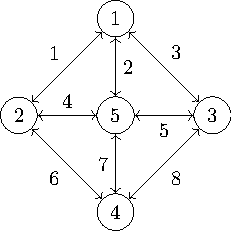
\includegraphics[keepaspectratio,width=1.0\textwidth,height=0.42\textheight]{chapters/tsp/figs/ugraph-figure0}
\caption{\label{fig:tsp:ugraph}Sample weighted graph G with at least one Hamiltonian cycle}
\end{figure}

Consider a digraph G such as that in \cref{fig:tsp:ugraph}.  Ordinarily this would be shown as an undirected graph because all arcs are two-way, but it is presented as an equivalent directed graph so that it more closely matches the input digraphs as described for the \gls{cps} rules described above, specifically regarding the set \(E\) of arc subcells.  A quick examination will show that there is at least one Hamiltonian cycle in this digraph, and thus there will be at least one Hamiltonian cycle with the minimum total weight.  \Cref{fig:tsp:utree} is a tree diagram showing the logical progression of the algorithm as applied to this digraph, assuming that vertex 1 is selected as the root of the Hamiltonian cycle.  Vertices in bold are the ends of the paths with a minimum cost, while vertices in italics are the ends of the paths where there is no arc in the digraph such that a Hamiltonian cycle can be completed, based on the digraph traversal up to that point.  The arcs are labelled with the cumulative weight of the path taken to reach the lower vertex.

\begin{figure}
\centering
% 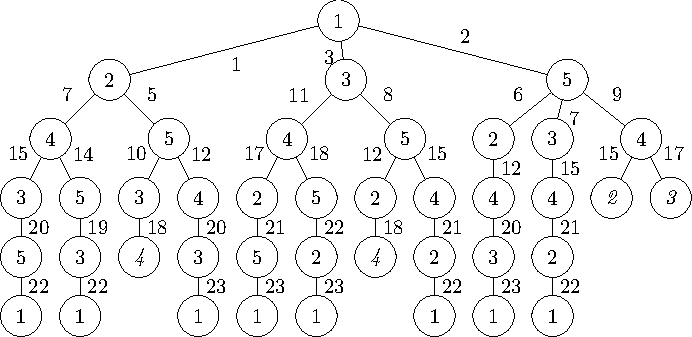
\includegraphics[keepaspectratio,width=1.0\textwidth,height=0.35\textheight]{chapters/tsp/figs/ugraph-figure1}
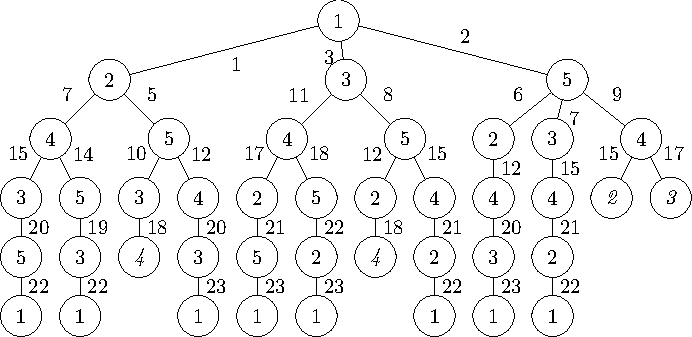
\includegraphics[keepaspectratio,width=1.0\textwidth]{chapters/tsp/figs/ugraph-figure1}
\caption[A tree diagram representing all potential evolutions of the \gls{cps} \glsentrylong{tsp-glossary} algorithm on the graph in \cref{fig:tsp:ugraph}]{\label{fig:tsp:utree}Tree diagram of the \gls{tsp} algorithm in action on graph G}
\end{figure}

\begin{cpobjectsfloat}
\begin{cpobjects}
    \cpobjectsline{\cpfunc{e}{\cpfunc{f}{1}\,\cpfunc{t}{2}\,\cpfunc{w}{1}} \; \cpfunc{e}{\cpfunc{f}{1}\,\cpfunc{t}{3}\,\cpfunc{w}{3}} \; \cpfunc{e}{\cpfunc{f}{1}\,\cpfunc{t}{5}\,\cpfunc{w}{2}} \; \cpfunc{e}{\cpfunc{f}{2}\,\cpfunc{t}{1}\,\cpfunc{w}{1}}}
    
    \cpobjectsline{\cpfunc{e}{\cpfunc{f}{2}\,\cpfunc{t}{4}\,\cpfunc{w}{6}} \; \cpfunc{e}{\cpfunc{f}{2}\,\cpfunc{t}{5}\,\cpfunc{w}{4}} \; \cpfunc{e}{\cpfunc{f}{3}\,\cpfunc{t}{1}\,\cpfunc{w}{3}} \; \cpfunc{e}{\cpfunc{f}{3}\,\cpfunc{t}{4}\,\cpfunc{w}{8}}}
    
    \cpobjectsline{\cpfunc{e}{\cpfunc{f}{3}\,\cpfunc{t}{5}\,\cpfunc{w}{5}} \; \cpfunc{e}{\cpfunc{f}{4}\,\cpfunc{t}{2}\,\cpfunc{w}{6}} \; \cpfunc{e}{\cpfunc{f}{4}\,\cpfunc{t}{3}\,\cpfunc{w}{8}} \; \cpfunc{e}{\cpfunc{f}{4}\,\cpfunc{t}{5}\,\cpfunc{w}{7}}}
    
    \cpobjectsline{\cpfunc{e}{\cpfunc{f}{5}\,\cpfunc{t}{1}\,\cpfunc{w}{2}} \; \cpfunc{e}{\cpfunc{f}{5}\,\cpfunc{t}{2}\,\cpfunc{w}{4}} \; \cpfunc{e}{\cpfunc{f}{5}\,\cpfunc{t}{3}\,\cpfunc{w}{5}} \; \cpfunc{e}{\cpfunc{f}{5}\,\cpfunc{t}{4}\,\cpfunc{w}{7}}}
    
    \cpobjectsline{\cpfunc{v}{\cpfunc{v}{1} \, \cpfunc{v}{2} \, \cpfunc{v}{3} \, \cpfunc{v}{4} \, \cpfunc{v}{5}}}
\end{cpobjects}
\caption[Starting set of subcells from \cref{fig:tsp:utree}]{\label{objs:tsp:obj1}Set of subcells from G in the skin membrane at the initial state}
\end{cpobjectsfloat}

The set of subcells contained inside the membrane at various points in the system's evolution are shown in \crefrange{objs:tsp:obj1}{objs:tsp:obj4} (for legibility, when specifying the \(p\) subcells, \cref{objs:tsp:obj4} adopts the compact presentation style for lists set out in \cref{sec:cps:lists}).  The system starts with the subcells shown in \cref{objs:tsp:obj1}, and the algorithm starts by applying \cpruleref{rule:tsp:tsp:start}, selecting vertex 1 as the starting point of the Hamiltonian cycle and creating the origin subcell \(\cpfunc{s}{\dots}\) (full details of the contents of the subcells are provided in the figures), as shown in \cref{objs:tsp:obj2}.

\begin{cpobjectsfloat}
\begin{cpobjects}
    \cpobjectsline{\cpfunc{e}{\cpfunc{f}{1}\,\cpfunc{t}{2}\,\cpfunc{w}{1}} \quad \cdots \quad \cpfunc{e}{\cpfunc{f}{5} \, \cpfunc{t}{4} \, \cpfunc{w}{7}}}
    \cpobjectsline{\cpfunc{s}{\cpfunc{r}{1} \; \cpfunc{u}{\cpfunc{v}{2} \, \cpfunc{v}{3} \, \cpfunc{v}{4} \cpfunc{v}{5}} \; \cpfunc*{p}{\cpfunc{h}{1} \cpfunc*{p}{\cpempty}} \; \cpfunc{c}{0}}}
\end{cpobjects}
\caption{\label{objs:tsp:obj2}Set of subcells in the skin membrane after the application of rule one}
\end{cpobjectsfloat}

Next, \cpruleref{rule:tsp:tsp:explore} is applied, creating the first level of subcells in the exploration tree.  This creates new \(\cpfunc{s}{\cpfunc{r}{R} \, \cpfunc{u}{\dots} \, \cpfunc{p}{\cpfunc{h}{\dots} \cpfunc*{p}{\cpfunc{h}{1} \cpfunc*{p}{\cpempty}}} \, \cpfunc{c}{\dots}}\) subcells, representing the potential paths of the cycle after one step.  \cpRuleref{rule:tsp:tsp:clean} concurrently removes the old \(s\) subcells from the system.  \Cref{objs:tsp:obj3} shows the subcells within the \gls{tlc} at the end of this first application of Rules \cpruleref*{rule:tsp:tsp:explore} and \cpruleref*{rule:tsp:tsp:clean}.

\begin{cpobjectsfloat}
\begin{cpobjects}
    \cpobjectsline{\cpfunc{e}{\cpfunc{f}{1}\,\cpfunc{t}{2}\,\cpfunc{w}{1}} \quad \cdots \quad \cpfunc{e}{\cpfunc{f}{5} \, \cpfunc{t}{4} \, \cpfunc{w}{7}}}
    \cpobjectsline{\cpfunc{s}{\cpfunc{r}{1} \; \cpfunc{u}{\cpfunc{v}{3} \, \cpfunc{v}{4} \cpfunc{v}{5}} \; \cpfunc{p}{\cpfunc{h}{2} \cpfunc*{p}{\cpfunc{h}{1} \cpfunc*{p}{\cpempty}}} \; \cpfunc{c}{1}}}
    \cpobjectsline{\cpfunc{s}{\cpfunc{r}{1} \; \cpfunc{u}{\cpfunc{v}{2} \, \cpfunc{v}{4} \cpfunc{v}{5}} \; \cpfunc{p}{\cpfunc{h}{3} \cpfunc*{p}{\cpfunc{h}{1} \cpfunc*{p}{\cpempty}}} \; \cpfunc{c}{3}}}
    \cpobjectsline{\cpfunc{s}{\cpfunc{r}{1} \; \cpfunc{u}{\cpfunc{v}{2} \, \cpfunc{v}{3} \cpfunc{v}{4}} \; \cpfunc{p}{\cpfunc{h}{2} \cpfunc*{p}{\cpfunc{h}{5} \cpfunc*{p}{\cpempty}}} \; \cpfunc{c}{2}}}
\end{cpobjects}
\caption{\label{objs:tsp:obj3}Set of subcells in the skin membrane after a single application of rules three and four}
\end{cpobjectsfloat}

Eventually, after repeating \cpruleref*{rule:tsp:tsp:explore} and \cpruleref*{rule:tsp:tsp:clean} four times, \cpruleref{rule:tsp:tsp:makezs} becomes applicable.  At this point, \cpruleref{rule:tsp:tsp:makezs} is applied, creating the \(z\) subcells that represent the final arc traversal from another vertex back to the origin vertex, vertex 1.  Finally, \cpruleref{rule:tsp:tsp:min} selects one of those \(z\) subcells with minimum cost as the solution, and outputs the path and cost subcells relating to that cycle.  \Cref{objs:tsp:obj4} outlines the subcells present in the system at this end point.

\begin{cpobjectsfloat}
\begin{cpobjects}
    \cpobjectsline{\cpfunc{e}{\cpfunc{f}{1}\,\cpfunc{t}{2}\,\cpfunc{w}{1}} \quad \cdots \quad \cpfunc{e}{\cpfunc{f}{5} \, \cpfunc{t}{4} \, \cpfunc{w}{7}}}
    \cpobjectsline{\cpfunc{z}{\cpfunc{c}{22} \; \cpfunc{p}{1|5|3|4|2|1}} \quad \cdots \quad \cpfunc{z}{\cpfunc{c}{22} \; \cpfunc{p}{1|2|4|3|5|1}}}
    \cpobjectsline{\cpfunc{c'}{22} \quad \cpfunc{p'}{1|5|3|4|2|1}}
\end{cpobjects}
\caption[Set of subcells in the skin membrane at completion of the computation]{\label{objs:tsp:obj4}Set of subcells in the skin membrane at completion of the computation, if \cpruleref{rule:tsp:tsp:min} selects the subcell containing the path subcell representing the traversals 1 - 2 - 4 - 3 - 5 - 1.}
\end{cpobjectsfloat}

To illustrate the progression of the algorithm through various branches of the exploration tree, consider the following examples, each beginning with the \(\cpfunc{s}{\ldots}\) and set of \(\cpfunc{e}{\ldots}\) subcells illustrated in \cref{objs:tsp:obj2}.

From \(\cpfunc*{s}{\cpfunc{r}{1}  \,\cpfunc*{u}{\cpfunc{v}{2}\,\cpfunc{v}{3}\,\cpfunc{v}{4}\,\cpfunc{v}{5}}\,  \cpfunc*{p}{\cpfunc{h}{1}\cpfunc{p}{\cpempty}}  \,\cpfunc{c}{0}}\), the subcell representing the beginning of the cycle at vertex 1, \cpruleref{rule:tsp:tsp:explore} will create, among others, an \(\cpfunc*{s}{\cpfunc{r}{1} \; \, \\ \allowdisplaybreaks \cpfunc*{u}{\cpfunc{v}{3} \, \cpfunc{v}{4} \, \cpfunc{v}{5}} \; \, \allowdisplaybreaks \cpfunc*{p}{\cpfunc{h}{2} \cpfunc*{p}{\cpfunc{h}{1} \cpfunc{p}{\cpempty}}} \; \, \allowdisplaybreaks \cpfunc{c}{1}}\) subcell representing an arc traversal to vertex 2 with a weight subcell \(\cpfunc{c}{1}\).  In turn, another new subcell, among others, will be derived from this subcell representing a further arc traversal to vertex 4, with a weight subcell of \(\cpfunc{c}{7}\).  This continues for subcells representing traversals to vertices 3 (\(\cpfunc{c}{15}\)) and 5 (\(\cpfunc{c}{20}\)), until finally the latter subcell contains an empty \(u\) subcell.  For this subcell, \cpruleref{rule:tsp:tsp:makezs} finds an \(e\) subcell that connects vertex 5 to \(R\), the root vertex 1, and so creates a \(z\) subcell (the top \(z\) subcell in \cref{objs:tsp:obj4}) containing a \(\cpfunc{p}{\dots}\) subcell representing the traversed path, and a subcell \(\cpfunc{c}{22}\), representing the total cost of the cycle.  This final subcell is potentially selected at random by \cpruleref{rule:tsp:tsp:min}, because 22 is the minimum cost possible in this particular digraph, when starting and finishing at vertex 1.

Conversely, another chain of subcell creations will occur as vertex 1 to vertex 5, with \(\cpfunc{c}{2}\), vertex 5 to vertex 4 with \(\cpfunc{c}{9}\), vertex 4 to vertex 2 with weight \(\cpfunc{c}{15}\).  At this point, \(\cpfunc{u}{\cpfunc{v}{3}}\) is non-empty, but there is no \(e\) subcell representing a transition from vertex 2 to vertex 3, so this subcell reaches a `dead-end', and will be removed without further effect by \cpruleref{rule:tsp:tsp:clean}.

Similarly, a progression will occur from vertex 1 to vertex 3 with \(\cpfunc{c}{3}\), to vertex 5 with \(\cpfunc{c}{8}\), to vertex 2 with \(\cpfunc{c}{12}\), and to vertex 4 with \(\cpfunc{c}{18}\).  At this point, every vertex has been visited, and the subcell \(u\) in this particular \(s\) subcell is empty, but there is no \(e\) subcell representing a transition from the current vertex back to the origin, so no \(z\) subcell will be created based on it.

%-------------------------------------------

\subsection{Directed Graph Example}
While the above example is drawn as a directed graph, to match better with the specification of the edges in the set of subcells \(E\), it was effectively an undirected graph.  To demonstrate that the \gls{tsp} algorithm is at least as effective in the directed case, \cref{fig:tsp:ugraph} was modified to remove some bidirectional arcs.  The modified digraph is presented in \cref{fig:tsp:digraph} and the accompanying exploration tree in \cref{fig:tsp:dtree}.  The updated set of subcells that are inside the skin membrane at the start of the computation are shown in \cref{objs:tsp:obj1d}.  The changes made are that the edges from 1 to 2 and from 5 to 3 have been removed, and the weights between 1 and 3 and 4 and 5 have been partially modified so that they are different in each direction.

\begin{figure}
\centering
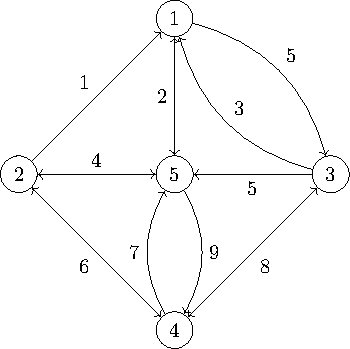
\includegraphics[keepaspectratio,width=1.0\textwidth,height=0.35\textheight]{chapters/tsp/figs/ugraph-figure2}
\caption{\label{fig:tsp:digraph}Sample weighted digraph H with at least one Hamiltonian cycle}
\end{figure}

\begin{figure}
\centering
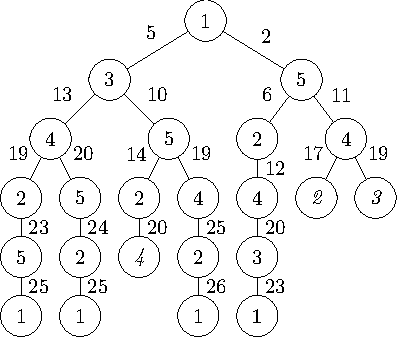
\includegraphics[keepaspectratio,width=1.0\textwidth,height=0.35\textheight]{chapters/tsp/figs/ugraph-figure3}
\caption[Tree diagram of the \glsentrylong{tsp-glossary} algorithm's operation on a directed graph]{\label{fig:tsp:dtree}Tree diagram of the \gls{tsp} algorithm in action on the second, directed graph, H}
\end{figure}

\begin{cpobjectsfloat}
\begin{cpobjects}
    \cpobjectsline{\mathbf{\cpfunc{e}{\mathbf{\cpfunc{f}{1}\,\cpfunc{t}{3}\,\cpfunc{w}{5}}}} \quad \cpfunc{e}{\cpfunc{f}{1}\,\cpfunc{t}{5}\,\cpfunc{w}{2}} \quad \cpfunc{e}{\cpfunc{f}{2}\,\cpfunc{t}{1}\,\cpfunc{w}{1}}}%
    \cpobjectsline{\cpfunc{e}{\cpfunc{f}{2}\,\cpfunc{t}{4}\,\cpfunc{w}{6}} \quad \cpfunc{e}{\cpfunc{f}{2}\,\cpfunc{t}{5}\,\cpfunc{w}{4}} \quad \cpfunc{e}{\cpfunc{f}{3}\,\cpfunc{t}{1}\,\cpfunc{w}{3}} \quad \cpfunc{e}{\cpfunc{f}{3}\,\cpfunc{t}{4}\,\cpfunc{w}{8}}}%
    \cpobjectsline{\cpfunc{e}{\cpfunc{f}{3}\,\cpfunc{t}{5}\,\cpfunc{w}{5}} \quad \cpfunc{e}{\cpfunc{f}{4}\,\cpfunc{t}{2}\,\cpfunc{w}{6}} \quad \cpfunc{e}{\cpfunc{f}{4}\,\cpfunc{t}{3}\,\cpfunc{w}{8}} \quad \cpfunc{e}{\cpfunc{f}{4}\,\cpfunc{t}{5}\,\cpfunc{w}{7}}}%
    \cpobjectsline{\cpfunc{e}{\cpfunc{f}{5}\,\cpfunc{t}{1}\,\cpfunc{w}{2}} \quad \cpfunc{e}{\cpfunc{f}{5}\,\cpfunc{t}{2}\,\cpfunc{w}{4}} \quad \mathbf{\cpfunc{e}{\mathbf{\cpfunc{f}{5}\,\cpfunc{t}{4}\,\cpfunc{w}{9}}}}}%
    \cpobjectsline{\cpfunc{v}{\cpfunc{v}{1} \, \cpfunc{v}{2} \, \cpfunc{v}{3} \, \cpfunc{v}{4} \, \cpfunc{v}{5}}}
\end{cpobjects}
    \caption[Set of subcells from H in the skin membrane at the initial state]{\label{objs:tsp:obj1d}Set of subcells from H in the skin membrane at the initial state (those different from G are in bold)}
\end{cpobjectsfloat}

These modifications have a significant effect upon the evolution of the system.  There are fewer potential paths through the digraph, which results in the instantiation of fewer subcells, and so the exploration tree is consequently narrower.  Thus, this particular application of the algorithm has a lower maximum space complexity.  Note though that there is absolutely no change in the operation of the algorithm.  The differences in the \(e\) subcells present at the start of the evolution of the system lead to a different result, without any change in the application of the rules.

%----------------------------------------
\section{\label{sect:variations}Variations on the Algorithms}
We have presented above algorithms to find a single Hamiltonian path or cycle, with minimum cost in the case of a weighted digraph (i.e., the \gls{tsp}).  With minimal modifications however, other results may be obtained from the algorithm, such as using a specific starting vertex or generating all possible paths/cycles.

To use a specific vertex as the starting point of the algorithm, rule (1) may be skipped by starting the system in state 2, with an \(s\) subcell containing the chosen vertex as the head of the \(p\) subcell supplied to the top-level cell.

For the \gls{hcp} and \gls{tsp}, rule (5) could be applied in \(\mathtt{max}\) mode without any other changes so as to produce all possible Hamiltonian cycles (with minimum cost for the \gls{tsp}) back to the starting node.  This results in the output into the top-level cell of multiple \(p'\) subcells, to be handled further as appropriate.  The same modification can be applied to rule (5) of the \gls{tsp} algorithm to obtain all minimum-cost cycle paths.  Likewise for each problem, if \(\mathtt{max}\) mode is used on rule (1), then the paths/cycles starting at every vertex will be generated.  These all potentially have the effect of increasing the space complexity of the system, which is not an issue for P~systems with their infinite available space, but may impact software simulations.

%In the case of a Hamiltonian path, more interesting is if a particular vertex is desired as the end point of the system.

% For the \gls{hcp} and \gls{tsp}, a specific vertex can be required as the ending point of the cycle.  This requires the instantiation of two extra unique subcells, which we will name here \(j\) and \(k\), shown in \autoref{hcprule12alt}.  Such a subcell is created either in the top-level cell at the time of application of rule (1), or supplied inside an initial \(s\) subcell.  Rule (2) of the \gls{hcp} or \gls{tsp} rules is modified so that instead of seeking \(e\) subcells that point back to the origin vertex, it instead instantiates the \(z\) subcells based on connections to the terminus vertex.  

% \begin{figure}[!htbp]
% \begin{framed}
% \renewcommand{\arraystretch}{1.5}
% \[\begin{array}{lllr}
% S_1 ~ & ~ v(v(R)v(N)Y) & \rightarrow_{1} ~ S_2 ~~ s(u(Y) ~ n(N) ~ p(h(R)p())) ~ & \qquad (1) \\
% S_2 ~ & ~   ~ &   \rightarrow_{1} ~ S_3 ~ p'(h(N)P)  & \qquad (2) \\
% 	~ & ~	~ & ~ \hspace{1.5cm} ~ | ~ s(u() ~ n(N) ~ p(h(N)P))	\\
% \end{array}\]
% \end{framed}
% \caption{Alternative rules 1 and 2 for the \gls{hcp} \& \gls{tsp} algorithms for finding cycles that end at a given vertex}
% \label{hcprule12alt}  
% \end{figure}

% For the \gls{hcp}, if all possible Hamiltonian cycles from the starting node are desired, rule (5) could instead be applied in \(\mathtt{max}\) mode without any other changes to achieve the desired result %, as shown in \autoref{hcprule5alt}
% -- this of course also applies to the \gls{hpp} rules.  This results in the output into the top-level cell of multiple \(p\) subcells, to be handled further as appropriate.
% %  Or rule (5) can leave the system in state \(S_3\), in which case the rule is applied ad infinitum, producing a path subcell at random from the collection of created subcells.  %Differently again, rule 5 could be modified so that it destroys the \(z\) subcell it selects instead of using it as a promoter, and thus the computation eventually terminates as all the generated \(z\) subcells are used up, but that appears to be simply a less efficient alternative to using \(\mathtt{max}\) mode.  
% The same modification can be applied to rule (5) of the \gls{tsp} algorithm to obtain all minimum-cost cycle paths.  Likewise, if \(\mathtt{max}\) mode is used on rule (1), then the paths/cycles starting at every vertex will be generated.

% \begin{figure}[!htbp]
% \begin{framed}
% \renewcommand{\arraystretch}{1.5}
% \[\begin{array}{lllr}
% S_3 ~ & ~   ~ & \rightarrow_{+} ~ S_4 ~ p'(P))   & \qquad \qquad (5b) \\
% 	~ & ~	~ & ~ \hspace{1.5cm} ~ | ~ z(p(P))	\\
% \end{array}\]
% \end{framed}
% \caption{Alternative rule 5 for the \gls{hcp} algorithm returning all Hamiltonian paths from a given starting node}
% \label{hcprule5alt}  
% \end{figure}

%Furthermore, if all possible Hamiltonian cycles from \textbf{every} node of the graph are desired, the only change required to achieve this is to modify rule (1) so that it operates in \(\mathtt{max}\) mode, rather than \(\mathtt{min}\) mode.  This would generate a starting \(s\) subcell carrying an \(r\) root subcell for every node in the graph, because the unification of \(R\) described in the rule will match upon every node contained in the initial \(v\) subcell.  Neither this change nor the alternative \(\mathtt{max}\)-mode rule (5) described above impact the running time of the algorithm -- though they will increase the space requirements to a greater or lesser degree, which has no effect in P~systems with their infinite available space, but may impact computerised simulations of them.

In \autoref{sect:algotsp} we assumed that all arc weights are strictly positive integers.  Weights of zero can be accommodated relatively easily.  Should every possible cycle have a minimum weight of at least 1, then no changes are needed.  If it is possible for there to be a cycle with a total weight of zero, then a sixth rule must be introduced, prior to the current rule (5), which in turn becomes rule (6).  This rule simply detects a minimum of zero, as set out in \autoref{sec-min}.  These new rules are shown in \autoref{minzerorules} (recall that \(\lambda\) inside a subcell denotes the subcell as empty).

% \begin{figure}[htbp]
% \begin{framed}
% %\begin{adjustwidth}{-1em}{-1em}
% \renewcommand{\arraystretch}{1.5}
% \[\begin{array}{lllr}
% % S_3 ~ & ~   ~ & \rightarrow_{1} ~ S_4 ~ p'(P) ~~~ c'(\lambda)  & (5) \\
% %     ~ & ~   ~ & ~ \hspace{1.5cm} ~ | ~ z(p(P) ~ c(\lambda)) \\
% % S_3 ~ & ~   ~ & \rightarrow_{1} ~ S_4 ~ p'(P) ~~~ c'(C1W)   & (6) \\
% % 	~ & ~	~ & ~ \hspace{1.5cm} ~ | ~ z(p(P) ~ c(C1W))	\\
% %     ~ & ~	~ & ~ \hspace{1.5cm} ~ \neg ~ z(p(\_) ~ c(C))	\\
% S_3 ~ & ~   ~ & \rightarrow_{1} ~ S_4 ~ p'(P) ~~~ c'(\lambda)  & (5) \\
%     ~ & ~   ~ & ~ \hspace{1.5cm} ~ | ~ z(p(P) ~ c(\lambda)) \\
% S_3 ~ & ~   ~ & \rightarrow_{1} ~ S_4 ~ p'(P) ~~~ c'(1D)   & (6) \\
% 	~ & ~	~ & ~ \hspace{1.5cm} ~ | ~ z(p(P) ~ c(1D))	\\
%     ~ & ~	~ & ~ \hspace{1.5cm} ~ \neg ~ (D = CW) ~ z(p(\_) ~ c(C))	\\
% \end{array}\]
% %\end{adjustwidth}
% \end{framed}
% \caption{Rules to find the minimum cost path in our \gls{tsp} algorithm, when that path cost may be zero}
% \label{minzerorules}  
% \end{figure}

\changerulenumber{4}

\begin{cprulesetfloat}
\begin{cpruleset}
    \cprule{s_3}{}{1}{s_4}{\cpfunc{p'}{P} \; \cpfunc{c'}{\cpempty}}
    \cppromoter{\cpfunc{z}{\cpfunc{p}{P} \, \cpfunc{c}{\cpempty}}}
    
    \cprule{s_3}{}{1}{s_4}{\cpfunc{p'}{P} \; \cpfunc{c'}{C \cpundig W}}
    \cppromoter{\cpfunc{z}{\cpfunc{p}{P} \, \cpfunc{c}{C \cpundig W}}}
    \cpinhibitor{\cpfunc{z}{\cpfunc{p}{\_} \, \cpfunc{c}{C}}}
    
\end{cpruleset}
\caption{\label{minzerorules} Rules to find the minimum cost path in our \gls{tsp} algorithm, when that path cost may be zero}
\end{cprulesetfloat}
\section{\label{sec:tsp:conc}Summary}
This chapter defined a succinct \gls{cps} algorithm for solving the \gls{tsp} in \bigoh{n} time, by using the capacity of \gls{cps} to create and manipulate complex subcells in only a few high-level steps.  This algorithm builds on a simpler version for finding Hamiltonian Paths and Cycles, requires only a fixed set of five rules, and takes \(n + 3\) steps to find a solution for any connected digraph of size \(n\), an improvement on the previous best known \gls{ps}-based solution to the \gls{tsp}.

Simple examples were provided to demonstrate the operation of the algorithm.  The \gls{tsp} algorithm can operate, without modification to the \gls{ruleset}, on any arbitrary weighted graph with a Hamiltonian Cycle.   The algorithm requires only a specification of the graph encoded as subcells, and could be extended to detect the absence of a Hamiltonian Cycle.

\begin{table}[htb]
\centering
\caption{Comparison of known exact \gls{ps} solutions to the \glsxtrlong{tsp}}
\label{tab:tsp:algocomp}
\setlength{\tabcolsep}{5pt}
\begin{tabular}{@{}lcc@{}}
\toprule
\textbf{Algorithm}  & \multicolumn{1}{l}{\textbf{\begin{tabular}[c]{@{}c@{}}Num. of\\  rules\end{tabular}}} & \multicolumn{1}{l}{\textbf{\begin{tabular}[c]{@{}c@{}}Run time\\  order\end{tabular}}} \\ \midrule
Guo \& Dai \cite{Guo2017}          & $\sim$50                                   & \bigoh{n^2}                                         \\
Cooper \& Nicolescu & 5                                          & \bigoh{n}                                          \\ \bottomrule
\end{tabular}
\end{table}

%-------------------------------------------------

% \begin{appendix}
\section{\label{sec:tsp:simulation}Simulations}
To demonstrate that this approach can be applied in practice to small problem graphs, sample simulations were written in SWI-Prolog, \fsharp{} and Erlang for the \gls{tsp} algorithm.  In each case, the programs were written with an emphasis on matching the \gls{cps} algorithm, rather than with a focus on memory or time efficiency.  Better implementations from a real-world-use viewpoint could likely be created, but they may not reflect the \gls{cps} rules quite as well.  The Prolog program in particular matches very closely to the \gls{cps} algorithm, and so is fully presented here.  A complete program listing for the Prolog program's rules corresponding to the algorithm is in \cref{app:tsp:codeprolog}, while \cref{app:tsp:probprolog} defines the problem graph.  A copy of the source code for each simulation is available at \url{https://github.com/jcoo092/cP-Systems-TSP}.  While care was taken to keep these simulations similar to each other, differences between the languages inevitably means they are not identical.

All three languages are reasonably well-suited to implementing \gls{cps}.  As mentioned, the Prolog program in particular maps well to the algorithm, requiring only 7 Prolog rules in total, plus a variable number of facts specifying the problem graph, 17 in this case.  The functional elements of \fsharp{} such as higher-order functions also allow a reasonable approximation, if perhaps not with quite the fidelity of Prolog.  Erlang, possibly owing to the fact it was originally implemented atop Prolog, appears to fall in between the two approaches, leaning more towards the functional side.  It is clear from these programs that there is at least one potential close mapping from \gls{cps} to both logic and functional programming languages.  The emphasis here, however, was on demonstrating the similarities of the languages to \gls{cps}, and not on performance.  As such, no attempt has been made to optimise the simulations.

To gauge their `real-world' effectiveness, the simulations were informally tested with increasing digraph sizes.  All three ably coped with digraph sizes of up to 10 vertices, returning an answer at most in a matter of a few seconds.  \fsharp{} and Erlang struggled somewhat at 11 vertices, with the latter taking more than one minute to complete, while Prolog quickly failed with an ``out-of-stack-memory'' error.  The \fsharp{} simulation was tested on a digraph of size 12, but the test was terminated after 90 minutes running time due to time constraints, failing to complete and return a minimum cost path.  Due to this, a 12 vertex run was not attempted with Erlang.

Considering that for a totally connected 11 vertex digraph, at the 11th step almost 40 million (\(11!\)) subcells would be required, it is unsurprising that memory limits may become an issue.  These results suggest that, while the fundamental process does indeed lead to determining lowest-cost paths, much more effective use of memory will be required to make software simulations practical for highly connected digraphs of any significant size (i.e. greater than approximately 11 or 12 vertices).

A comparison of \cref{fig:tsp:utree,fig:tsp:dtree} suggests, however, that for graphs that are not totally connected, the implementations may cope much better, as would be expected.  With ultimately fewer paths to explore, the growth in the number of objects will be lesser, and thus the space requirements will be lowered.  This is not unique by any means to the \gls{cps} version of the \gls{tsp} - any method to solve the \gls{tsp} which involves a breadth-first search of the graph, considering whether nodes have already been visited, will experience the same. 

\subsection{Prolog simulation}

It is perhaps interesting to contrast the Prolog method for exploring the problem space and finding an answer with that of \gls{cps}.  On the surface they appear quite similar -- a handful of rules and some initial statements specific to the problem, combined with unification.   In some ways, however, they appear also to be opposing duals of each other.  Prolog in general, and thus in the case of this program, works on a top-down backward-chaining approach, whilst \gls{cps} works on a bottom-up forward-chaining approach.

That is to say that (sequential) Prolog tries to do the least work and use the least space possible, so it starts with the definition of the requested inference (an invocation of \texttt{go} in the program), and only evaluates elements of that definition as it discovers they are needed in order to provide a result.  In the case of the digraph exploration, this essentially means that it tries to perform a linear depth-first search of the digraph, stopping as soon as it has an answer --- though with the \gls{tsp} it inevitably must evaluate every cycle to know which has minimum cost.

Conversely, the \gls{cps} algorithm starts with the definition of the problem graph, and does all possible work in order to find the result in what is essentially a breadth-first search.  All possible cycles from the root node are instantiated and eventually checked for minimum cost. The ability of \gls{cps} to perform these instantiations and the comparison completely in parallel means that a relatively small number of steps are required to find the minimum -- though at the cost of a potentially (exponentially) large space and processing complexity.

\begin{listing}
\caption{\label{app:tsp:probprolog}SWI-Prolog code defining the example problem undirected graph G shown in \cref{fig:tsp:ugraph}}
\inputminted[linenos,breaklines,frame=lines,autogobble,lastline=3]{prolog}{chapters/tsp/code/tsp.pl.txt}
\end{listing}

\begin{listing}
\caption[Complete SWI-Prolog code for the \acrlong{tsp} algorithm]{\label{app:tsp:codeprolog}Complete SWI-Prolog code for the rules of the \gls{tsp} algorithm}
\inputminted[linenos,breaklines,frame=lines,autogobble,firstline=5]{prolog}{chapters/tsp/code/tsp.pl.txt}
\end{listing}
% \end{appendix}
